\subsection{The readout plane is not flat: a bow of the readout boards}\label{sec:bow}
\sectionstate{partial}{model-audit follow-up FB, \texttt{rerun/model\_audit/followups/fb\_bow\_maps/} (2026-10-27); slide note \texttt{notes/mx17-chamber-bow}}
\intent{Establish, from bench data alone, that the mesh surface of every chamber is dished by 1--3\,mm and that the drift
direction follows its slope; give its size per chamber, its sign from external facts, how stable it is, the evidence
that excludes the alternatives, and what correcting for it gains. Draft (2026-10-27).}

A micro-TPC converts the time structure of the induced signals into a track angle under two assumptions about the
chamber: that the readout plane is flat and that the drift field is perpendicular to it. On all five chambers measured on
the cosmic bench, both assumptions fail at the millimetre level, in the way a bowed readout board predicts.

\paragraph{Three independent observables.}
(i)~\emph{Positions.} A track of slope $\tan\theta = \mathrm{d}x/\mathrm{d}z$ crosses a mesh displaced by $h$ along $z$
at a point shifted by $h\tan\theta$. In every position cell the slope of the position residual (fitted mesh position
minus the M3 prediction) against the M3 slope is therefore the local mesh height $h(x,y)$. It is measured independently
by the X and the Y strips, through the two independent M3 projections. Both views see a dish in both directions
(Fig.~\ref{fig:bowprof}): the centre lies $1.5$--$2.3$\,mm below a point 150\,mm out along either axis
(det2 $1.8\pm0.2$, det3 $1.5\pm0.2$, det4 $1.9\pm0.2$, det6 $1.8\pm0.2$, det7 $2.3\pm0.4$\,mm), i.e.\ a curvature of
$1.3$--$2.1\times10^{-4}$\,mm$^{-1}$.
(ii)~\emph{Drift tilt.} If drift lines leave the mesh normal to its surface, charge produced at height $d$ arrives
displaced by $d\,\partial h/\partial x$, so the fitted transverse speed acquires an offset
$w_0 = v\,r_f\,\partial h/\partial x$ with $r_f$ between $1/2$ (flat cathode) and 1 (cathode bowed with the board).
For a dish, $w_0$ must rise linearly across the chamber. It does, in all ten chamber views, by
$\pm0.6$\,\textmu m/ns over 300\,mm, with $r_f = 0.4$--$0.9$ on nine of ten views (Fig.~\ref{fig:bowclos}). The
sign of this relation is predicted by the geometry, not fitted.
(iii)~\emph{Narrowest cluster.} The cluster of strips above threshold is narrowest for the track running along the
local drift lines, at $\tan\theta = -w_0/v$. This uses amplitudes only, with no hit times and no fitted angle; the
narrowest-cluster slope drifts across the chamber with the predicted sign on 9/10 views.

\paragraph{Sign.}
The M3 $z$ axis points up (the ray files carry the top and bottom M3 plane heights, 1302 and 24\,mm; the upper DUT slot
is at 702\,mm, the lower at 232\,mm), and the chambers lie with the readout board down and the cathode up (the fitted
micro-TPC slope has the sign of the M3 slope on every chamber). The mesh centre is therefore \emph{lower} than its rim,
further from the cathode: the direction in which the board's weight, gas overpressure and residual mesh tension all push.

\paragraph{Alternatives.}
A plane-scale error of the telescope that could produce the $w_0$ ramp would leave a $\sim$6\,\% position scale at the
chamber; the measured residual scale is below 0.15\,\%. A position-dependent $t_0$ bias would vanish when every track is
moved to a fixed trigger latency; 80--100\,\% of the curvature survives. Fringe fields at the frame decay within
$\sim$10\,mm of the edges, while the ramp is linear over 300\,mm. A bow of the M3 planes would shift tracks by
$\tan\theta\, g(x,y)$ and can mimic $h$, but cannot produce $w_0$ or move the narrowest cluster; a common telescope
contribution to the depth cannot be excluded and limits the depth to $0.5$--$1.3$ times the quoted value.
The column duration, which should lengthen where the gap deepens, does not resolve the effect: its X and Y readings of
the same column differ by more than the 1--2\,mm expected.

\paragraph{Stability.}
Nineteen bench runs were reconstructed with each chamber's own calibration and their own alignment: other subruns of
the same night, other nights (det2 after a remount, det3 and det4 on other days), both bench slots (det3 at $z=702$ and
$232$\,mm) and other drift and mesh voltages. Fifteen give their chamber's dish depth within $2\sigma$; the one clear
outlier is det3 on 6-25 ($0.9\pm0.1$\,mm against a det3 mean of $\approx1.5$\,mm), while det3 in the same lower slot on
6-23 reads $1.7\pm0.1$\,mm. The drift-tilt shape measured on one run, applied to the others with only the rigid tilt
re-measured, recovers a median 94\,\% of the angular-resolution gain of each run's own map. The bow is therefore a
static property of each chamber at the 20\,\% level; which load sets it cannot be separated with the data available.

\paragraph{Plausibility.}
The 1.7\,mm readout PCB spans the 0.40\,m aperture of its support plate with only 5\,mm of Rohacell behind it. A
Kirchhoff-plate estimate gives a dip at 150\,mm of 0.1--0.25\,mm from its own weight, 0.3--0.7\,mm per mbar of gas
overpressure and up to $\sim$1\,mm from a mesh laminated under 10\,N/cm: the measured depth needs no exotic load.

\paragraph{Correction.}
The bow enters the reconstruction only through the conversion of the fitted transverse speed into an angle and through
the height of the track point. A per-chamber surface (static shape) plus the per-run rigid tilt, validated by two-fold
cross-validation on held-out tracks, improves the angular resolution by a median of 16\,\% (1--30\,\% per view); the
shape predicted from positions alone, with two numbers fitted to the angles, recovers 15\,\%. With the final reconstruction settings (one prompt footprint $\sigma_0=0.30$\,mm for both views, pinned $t_0$, 20\,ns grid) the same map still improves the Y-view resolution by 13--25\,\% and removes a $-8$\,\% steep-track compression on det6\,X. Subtracting
$h\tan\theta$ improves the position residual by 4--15\,\%. Because the load depends on mounting and the chambers
stand vertical at n\_TOF, the bench surface is not transferred to the beam data without an in-situ measurement.
\askDylan{Is a direct flatness measurement of a spare board (or the photographs of the opened chambers) available to
quote alongside? No new data are needed for the text as it stands.}

\begin{figure}[t]
  \centering
  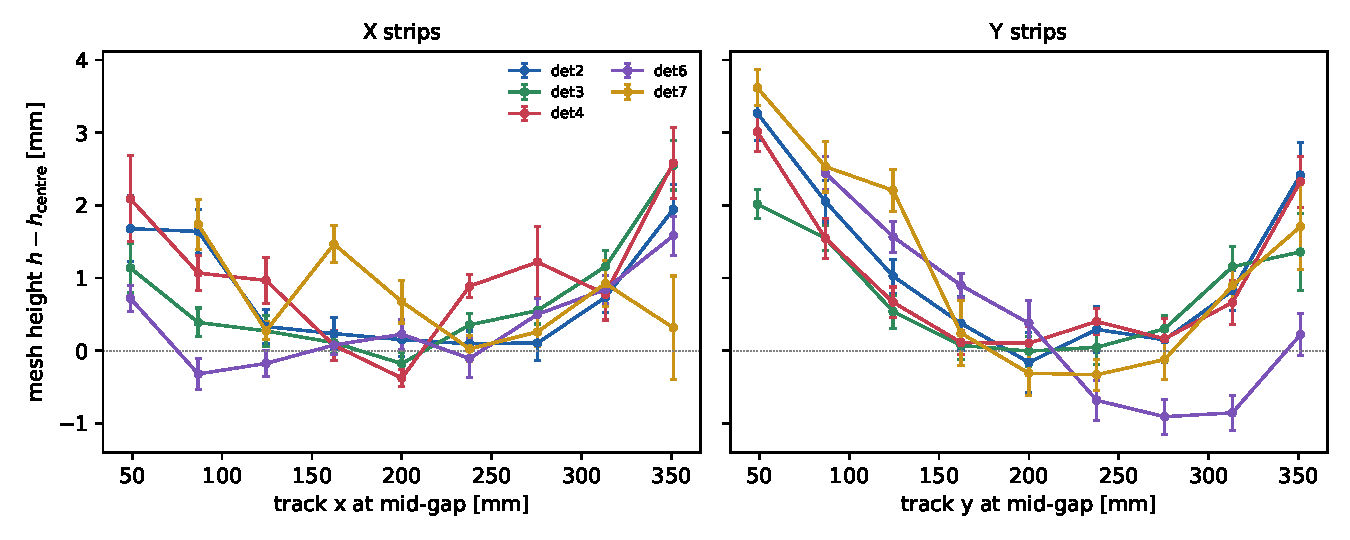
\includegraphics[width=0.95\linewidth]{bow_profiles}
  \caption{Mesh height across the chamber from position residuals against the M3 track slope, for the X (left) and Y
  (right) strips of the five chambers, relative to the fitted parabola's value at the centre. Golden bench rows.}
  \label{fig:bowprof}
\end{figure}
\begin{figure}[t]
  \centering
  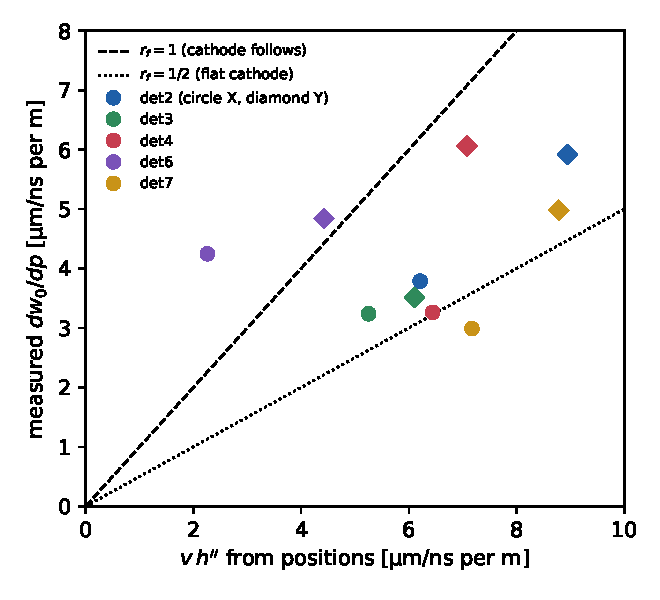
\includegraphics[width=0.5\linewidth]{bow_closure}
  \caption{Gradient of the drift-tilt offset $w_0$ across the chamber against the gradient predicted from the
  position-route curvature, $v\,h''$. Lines: drift lines tilted fully with the mesh ($r_f=1$) and a flat cathode
  ($r_f=1/2$). Circles X strips, diamonds Y strips.}
  \label{fig:bowclos}
\end{figure}
